\lab{Lorenz Equations}{Lorenz Equations}
% \epigraph{\textit{Chaos: When the present determines the future, but the approximate present does not approximately determine the future.}}{Edward Lorenz}
\objective{Investigate the behavior of a system that exhibits chaotic behavior.
Demonstrate methods for visualizing the evolution of a system.}
\labdependencies{Animation,IVPBVPIntro}

Chaos is everywhere.
It can crop up in unexpected places and in remarkably simple systems, and a great deal of work has been done to describe the behavior of chaotic systems.
One primary characterization of chaos is that small changes in initial conditions result in large changes over time in the solution curves.

\section*{The Lorenz System}
One of the earlier examples of chaotic behavior was discovered by Edward Lorenz.
In 1963, while working to study atmospheric dynamics, he derived the simple system of equations
\begin{align*}
\frac{d x}{d t} &= \sigma \left(y - x\right) \\
\frac{d y}{d t} &= \rho x - y - x z \\
\frac{d z}{d t} &= x y - \beta z
\end{align*}
where $\sigma$, $\rho$, and $\beta$ are all constants.
After deriving these equations, he plotted the solutions and observed some unexpected behavior.
For appropriately chosen values of $\sigma$, $\rho$, and $\beta$, the solutions did not tend toward any steady fixed points, nor did the system permit any stable cycles.
The solutions did not tend off toward infinity either.
This began the study of what was called a \textit{strange attractor}.
Although relatively simple, this system exhibits chaotic behavior.

\begin{comment}
\subsection*{Plotting and Interacting}
We will be making interactive 3D plots using \li{matplotlib}.
Please refer back to the \textit{Introduction to Matplotlib} lab for tips and tricks to graphing 3D.
Below is some sample code to help you out.

\begin{lstlisting}
from matplotlib import rcParams, pyplot as plt

rcParams['figure.figsize'] = (16,10)     #Affects output size of graphs.
'''
Code up your X, Y, Z values
'''
fig = plt.figure()
ax = fig.gca(projection='3d')
ax.plot( X, Y, Z )    #Make sure X, Y, Z are same length.
                      #Connect points (X[i], Y[i], Z[i]) for i in len(X)
ax.set_xlabel('X')
ax.set_ylabel('Y')
ax.set_zlabel('Z')

ax.set_xlim3d([min(X), max(X)])    #Bounds the axes nicely
ax.set_ylim3d([min(Y), max(Y)])
ax.set_zlim3d([min(Z), max(Z)])

plt.show()
\end{lstlisting}

Because we are plotting in 3D, we are also interested in being able to interact with the plot and rotate it to analyze what our solutions are actually doing.
To facilitate this, \li{matplotlib} has different backends which allow for various levels of control over what our graphs do.
These backends are accessed using \li{matplotlib}'s \li{switch_backend()} function with a call to whichever backend we want.
Your computer may default to a backend which you can already interact with (try clicking your plot and rotating it to see).
If not, consider using 'qt5agg', 'qt4agg', nbagg', or 'tkagg' in the function call.

\begin{lstlisting}
plt.switch_backend('qt5agg') # This backend opens the graph in a new window
\end{lstlisting}

\begin{warn}
Do not run \li{\%matplotlib inline} with this code. You will crash your kernel.
\end{warn}
\end{comment}

\begin{problem}
Write a function that implements the Lorenz equations. Let $\sigma=10$, $\rho=28$, $\beta=\frac{8}{3}$. 
Make a 3D plot of a solution to the Lorenz equations, where the initial conditions $x_0,y_0,z_0$ are each drawn randomly from a uniform distribution on $[-15,15]$ and for \(t\) in the range \([0,25]\). 
As usual, use \li{scipy.integrate.solve_ivp} to compute an approximate solution. 
Compare your results with Figure \ref{fig:Single_Lorenz}.
\end{problem}


\begin{figure}
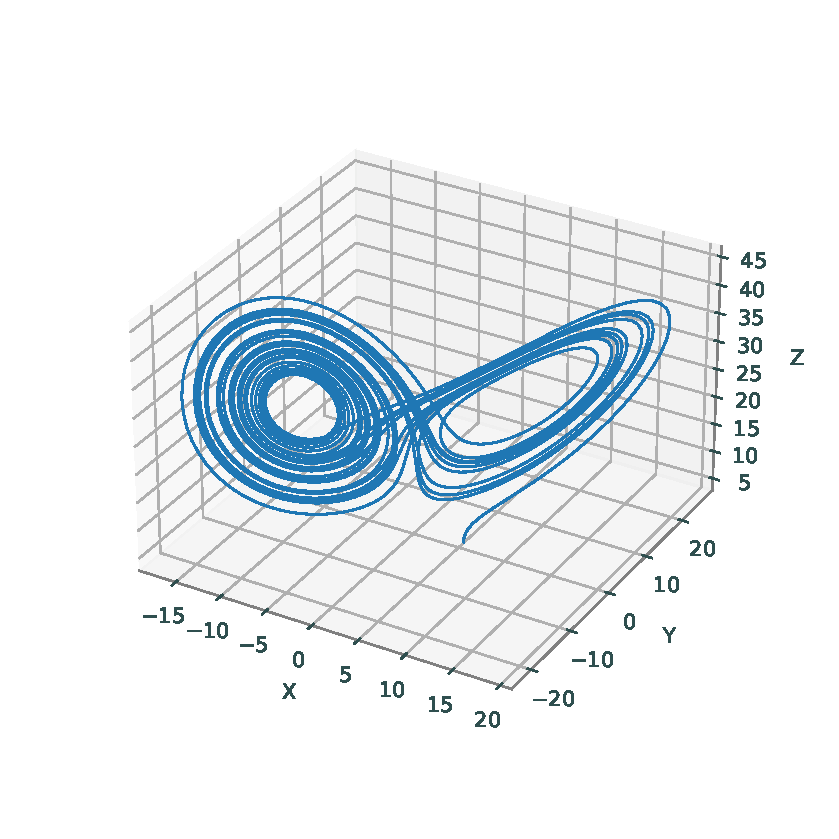
\includegraphics[width=\textwidth]{figures/Single_Lorenz.pdf}
\caption{Approximate solution to the Lorenz equation with random initial conditions}
\label{fig:Single_Lorenz}
\end{figure}

\section*{Basin of Attraction}
Notice in the first problem that the solution tended to a certain region, called an \textit{attractor}. 
The \textit{basin of attraction} of an attractor is the set of initial conditions that tend towards the attractor.
We will investigate the basin of attraction of the Lorenz system by changing the initial conditions.
\begin{problem}
To better visualize the Lorenz attractor, produce a single 3D plot displaying three solutions to the Lorenz equations, each with random initial conditions as before. 
Compare your results with Figure \ref{fig:Multiple_Lorenz}.
\end{problem}

\begin{figure}
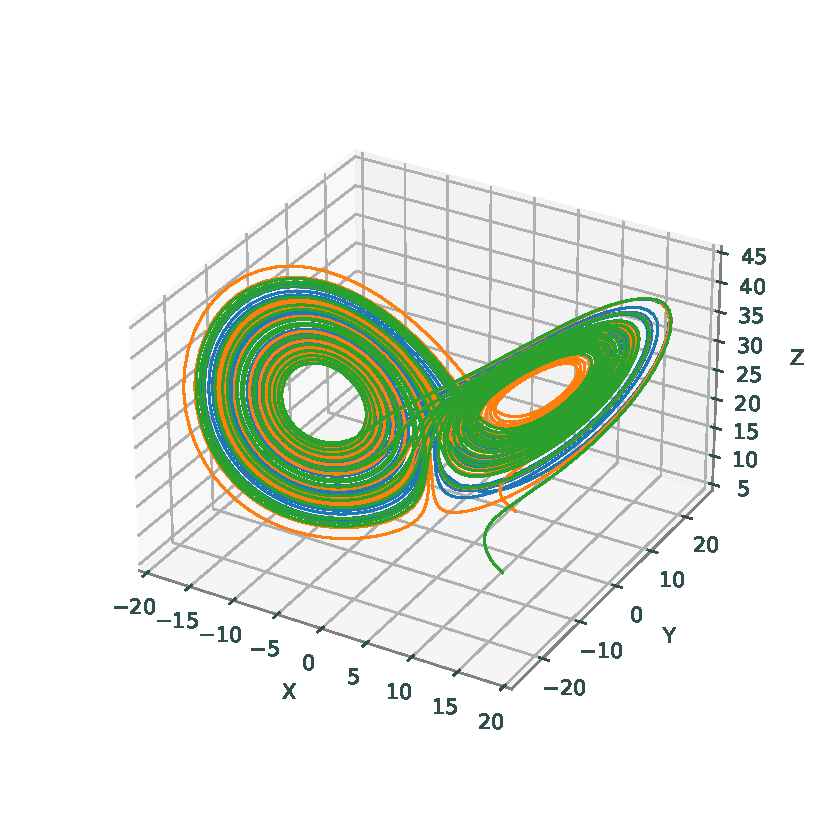
\includegraphics[width=\textwidth]{figures/Multiple_Lorenz.pdf}
\caption{Multiple solutions to the Lorenz equation with random initial conditions}
\label{fig:Multiple_Lorenz}
\end{figure}

\section*{Chaos}
Chaotic systems exhibit high sensitivity to initial conditions. 
This means that a small difference in initial conditions will generally result in solutions that diverge significantly from each other. 
However, chaotic systems are not \textit{random}. 
An explanation given by Lorenz is that chaos is "when the present determines the future, but the approximate present does not approximately determine the future."

\begin{problem}
\label{lorenz:prob:chaos}
Use \li{matplotlib.animation.FuncAnimation} to produce a 3D animation of two solutions to the Lorenz equations with nearly identical initial conditions. To make the initial conditions, draw $x_0,y_0,z_0$ as before, and then make a second initial condition by adding a small perturbation to the first (try using \li{np.random.randn(3)*(1e-8)} for the perturbation). Note that it may take several seconds before the separation between the two solutions will be noticeable. Evaluate on \li{t_span=(0,50)} and use the \li{t_eval} argument of \li{solve_ivp}, with \li{t_eval=np.linspace(0,50,3000)}. Using this argument causes \li{solve_ivp} to return the solution's values at the points you pass in.

The animation should display a point marker as well as the past trajectory curve for each solution. 
Save your animation as \li{lorenz_animation1.mp4}.
\end{problem}

In a chaotic system, round-off error implicit in a numerical method can also cause divergent solutions. For example, using a Runge-Kutta method with two different values for the stepsize $h$ on identical initial conditions will still result in approximations that differ in a chaotic fashion.

\begin{comment}
\begin{figure}
\includegraphics[width=\textwidth]{figures/perturbed_lorenz.pdf}
\caption{Two solutions to the Lorenz equation with perturbed initial conditions}
\label{fig:perturbed_lorenz}
\end{figure}

You may be wondering if your code was even correct.
You could distinctly see the two curves because there was some separation of color, but who is to say that the two solutions moved away from each other only slightly as time went on.
Our next task will be to \textit{animate} this beast.

\section*{Intro to Animation}
Let's get you a degree in Computer Animation.
You will be provided with some code that helps with animation.
Please feel free to play around and try to animate different things.
Again, refer to the \textit{Introduction to Matplotlib} lab for additional help.

We will call on \li{matplotlib.animate} to assist in animation. Import the following:
\begin{lstlisting}
from matplotlib.animation import FuncAnimation
\end{lstlisting}
Follow these steps for setting up an animation.
\begin{itemize}
\item Calculate all data needed for the animation (not necessary in some cases, but it simplifies things).
\item Define a figure explicitly with \li{plt.figure()} and set its window boundaries.
\item Draw empty objects that can be altered dynamically.
\item Define a function to update the drawing objects.
\item make a call to \li{FuncAnimation()} which will start the animation.
\end{itemize}
\li{FuncAnimation()} accepts the figure to be animated, the function that updates the figure, the number of frames to show before repeating, and how fast to run the animation (lower number $=$ faster).

Check out the sample code for animating two 2D objects simultaneously.
\begin{lstlisting}
from matplotlib.animation import FuncAnimation

def sine_cos_animation():
	#Calculate the data to be animated
	x = np.linspace(0, 2*np.pi, 200)[:-1]
	y1, y2 = np.sin(x), np.cos(x)
	
	#Create a figure and set the window boundaries
	fig = plt.figure()
	plt.xlim(0, 2*np.pi)
	plt.ylim(-1.2, 1.2)
	
	#Initiate empty lines of the correct dimension
	sin_drawing, = plt.plot([], [])
	cos_drawing, = plt.plot([], [])	#note the comma after the variable name
	
	#Define a function that updates each line
	def update(index):
		sin_drawing.set_data(x[:index], y1[:index])
		cos_drawing.set_data(x[:index], y2[:index])
		return sin_drawing, cos_drawing,
	
	a = FuncAnimation(fig, update, frames=len(x), interval=10)
	plt.show()
\end{lstlisting}

\begin{warn}
The above animation code works great for 2D animations, but \li{set_data()} is only good for 2D. When you want to animate in 3D, you will need an extra empty list in \li{plt.plot()} and a call to \li{set_3d_properties()} in the \li{update(index)} function.
\end{warn}

\section*{Animate}
You now know how to plot the Lorenz equation, how to plot multiple equations, and even how to animate (yay you, you're a star) simple plots.
It's time to put all your know-how to good use.
\end{comment}

\begin{problem}
Even differences due to small numerical errors can cause solutions of chaotic systems to diverge from each other.
The \li{solve_ivp} function allows user to specify error tolerances (similar to setting a value of $h$ in a Runge-Kutta method). 
Using a single initial condition, produce two approximations by using the \li{solve_ivp} arguments \li{(atol=1e-15, rtol=1e-13)} for the first approximation and \li{(atol=1e-12, rtol=1e-10)} for the second.

As in the previous problem, use \li{FuncAnimation} to animation both solutions. Save the animation as \li{lorenz_animation2.mp4}. Use the same \li{t_span} and \li{t_eval} arguments as in problem \ref{lorenz:prob:chaos}.
\end{problem}

\begin{comment}
If our system is very chaotic, then even small round off errors in your computer can lead to drastically different solutions.

\begin{problem}
Now set one initial condition.
Use \li{solve_ivp} to solve the system, but use the arguments \li{atol=1E-14}, \li{rtol=1E-12}, and then again with \li{atol=1E-15}, \li{rtol=1E-13}.
Animate both solutions on the same plot.
\end{problem}
\end{comment}

\section*{Lyapunov Exponents}
The \textit{Lyapunov exponent} of a dynamical system is one measure of how chaotic a system is.
While there are more conditions for a system to be considered chaotic, one of the primary indicators of a chaotic system is \textit{extreme sensitivity to initial conditions}.
Strictly speaking, this is saying that a chaotic system is poorly conditioned.
In a chaotic system, the sensitivity to changes in initial conditions depends expoentially on the time the system is allowed to evolve.
If $\delta(t)$ represents the difference between two solution curves, when $\delta(t)$ is small, the following approximation holds.
\[\|\delta(t)\| \sim \|\delta(0)\| e^{\lambda t}\]
where $\lambda$ is a constant called the Lyapunov exponent. In other words, $\log(\|\delta(t)\|)$ is approximately linear as a function of time, with slope $\lambda$.
For the Lorenz system (and for the parameter values specified in this lab), experimentally it can be verified that $\lambda \approx .9$.

\begin{figure}
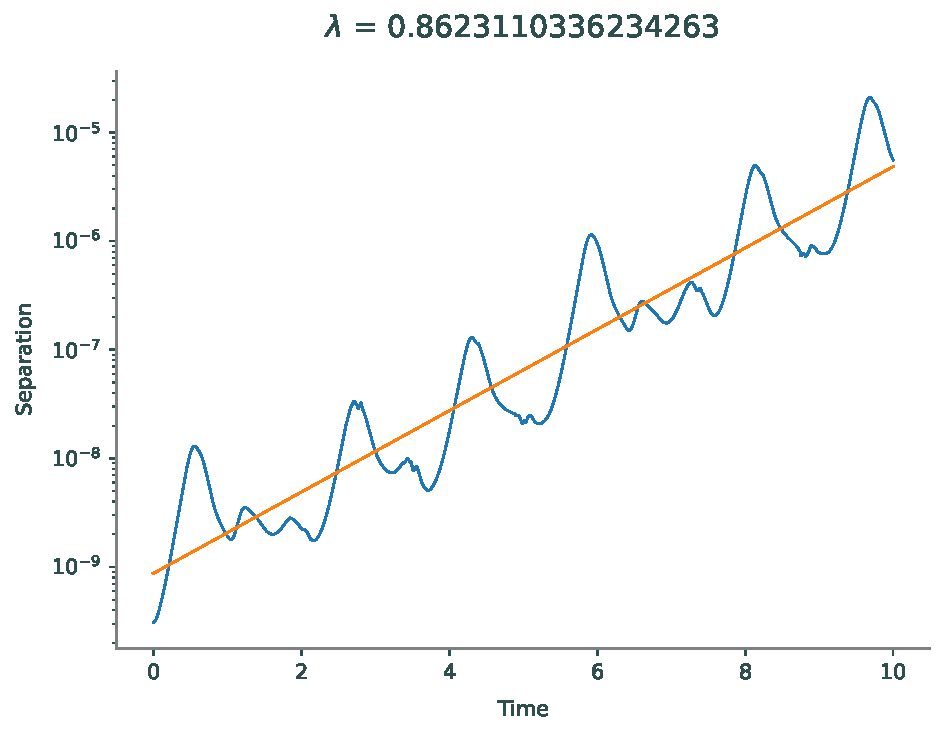
\includegraphics[width=\textwidth]{figures/semilog.pdf}
\caption{A semilog plot of the separation between two solutions to the Lorenz equations together with a fitted line that gives an estimate of the Lyapunov exponent of the system.}
\label{fig:lyapunov_exponent}
\end{figure}

\begin{comment}
Suppose we want tol find the Lyapunov exponent for the Lorenz System.
Start by importing \li{linalg} and \li{linregress} modules from \li{scipy}.
\begin{lstlisting}
from scipy import linalg as la
from scipy.stats import linregress
\end{lstlisting}
To get a good estimate of the Lyapunov exponent, we want to make sure our initial solution already lies on the attractor.
To do this, choose some random initial conditions, run your \li{solve_lorenz} function, then pick out the final coordinates.
Let these coordinates be the starting point for our next system.

Next perturb the conditions slightly.
Find the solution curve using these two sets of initial coordinates and then calculate the \li{norm} between the solution at each point.
Plot the norm using \li{plt.semilogy(time, norm)}.

Finally we want to calculate the exponential line fitted to the data.
Because we are using the semilog plot, we can find this line as follows:
\begin{itemize}
\item take the \li{log} of the norms.
\item use \li{linregress()} to compute the linear regression of the log of the norms.
\item take the \li{exp} of the linear regression to turn back into an exponential regression.
\item plot the exponential regression using \li{plt.semilogy()} (your solution will be a line)
\end{itemize}
\end{comment}


\begin{problem}
Estimate the Lyapunov exponent of the Lorenz equations by doing the following:
\begin{itemize}
	\item Produce an initial condition that already lies in the attractor. This can be done by using a random "dummy" initial condition, approximating the resulting solution to the Lorenz system for a short time, and then using the endpoint of that solution (which is now in the attractor) as the desired initial condition.
	\item Produce a second initial condition by adding a small perturbation to the first (as before).
	\item For both initial conditions, use \li{solve_ivp} to produce approximate solutions for $0 \leq t \leq 10$.
	\item Compute $\|\delta(t)\|$ by taking the norm of the vector difference between the two solutions for each value of $t$.
	\item Use \li{scipy.stats.linregress} to calculate a best-fit line for $\log(\|\delta(t)\|)$ against $t$.
	\item The slope of the best-fit line is an approximation for the Lyapunov exponent $\lambda$.
	
\end{itemize}
Produce a plot similar to Figure \ref{fig:lyapunov_exponent} by using \li{plt.semilogy}. 

Hint: Remember that the best-fit line you calculated corresponds to a best-fit exponential for $\|\delta(t)\|$. If \li{a} and \li{b} are the slope and intercept of the best-fit line, the best-fit exponential can be plotted using \li{plt.semilogy(t,np.exp(a*t+b))}. Use the \li{t_eval} argument of \li{solve_ivp} (as in problem \ref{lorenz:prob:chaos}) for both solutions to the Lorenz equation so that you can compute $\|\delta(t)\|$ for the same time steps.
	

\end{problem}